\documentclass[border=10pt]{standalone}
\usepackage{tikz}

\begin{document}

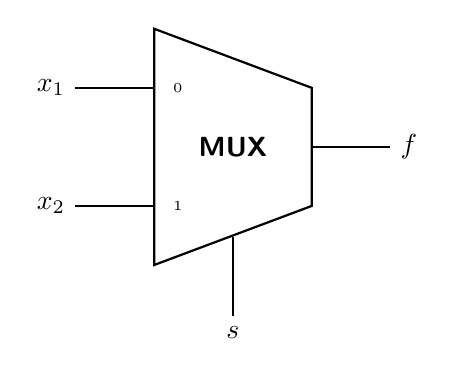
\begin{tikzpicture}
    % --- Configuration ---
    % You can adjust these widths/heights
    \def\width{2}       % Width of the MUX
    \def\heightL{3}     % Height of the left side (Input side)
    \def\heightR{1.5}   % Height of the right side (Output side)
    
    % --- Draw the Body (Trapezoid) ---
    % Coordinates calculated based on center at (0,0)
    \draw[thick, fill=white] 
        (-\width/2, \heightL/2) coordinate (TopLeft) -- 
        (\width/2, \heightR/2) coordinate (TopRight) -- 
        (\width/2, -\heightR/2) coordinate (BotRight) -- 
        (-\width/2, -\heightL/2) coordinate (BotLeft) -- 
        cycle;

    % --- Label the Body ---
    \node at (0,0) {\sffamily\bfseries MUX};

    % --- Draw and Label Inputs (x1, x2) ---
    % Input 1 (Top)
    \draw[thick] (-\width/2, \heightL/4) -- ++(-1,0) node[anchor=east] {$x_1$};
    % Input 2 (Bottom)
    \draw[thick] (-\width/2, -\heightL/4) -- ++(-1,0) node[anchor=east] {$x_2$};

    % --- Draw and Label Output (f) ---
    \draw[thick] (\width/2, 0) -- ++(1,0) node[anchor=west] {$f$};

    % --- Draw and Label Select (s) ---
    % Drawn from the bottom edge
    \draw[thick] (0, -1.15) -- ++(0,-1) node[anchor=north] {$s$};
    
    % Optional: Add port numbers inside (0, 1)
    \node[font=\tiny] at (-\width/2 + 0.3, \heightL/4) {0};
    \node[font=\tiny] at (-\width/2 + 0.3, -\heightL/4) {1};

\end{tikzpicture}

\end{document}